\documentclass[tikz,border=5mm]{standalone}
\usepackage{calc}
\begin{document}
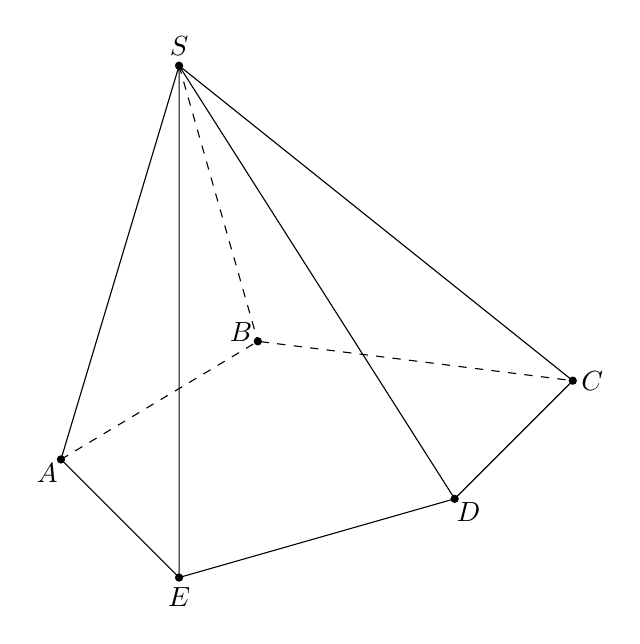
\begin{tikzpicture}[declare function={h=5;}]
		\path (0,0) coordinate (A)
		(1.5,-1.5) coordinate (E)
		(5,-0.5) coordinate (D)
		(6.5,1) coordinate (C)
		(2.5,1.5) coordinate (B)
        (1.5, h) coordinate (S);
		\draw[dashed] (A)--(B)--(C) (S)--(B);
		\draw (A)--(E)--(D)--(C)--(S)--(A) (S)--(E) (S)--(D);
		\foreach \x/\g in {S/90,B/150,A/-135,E/-90,D/-45,C/0}{
		    \fill (\x) circle (1.5pt)+(\g:7pt) node{$\x$};
		}
\end{tikzpicture}
\end{document}
